
Para obtener una herramienta que pueda ser utilizadas desde
Mumuki es necesario cumplir con ciertas pautas a la hora
de interactuar con la plataforma.

\subsection{Requerimientos de la Plataforma}

La Plataforma Mumuki se puede entender desde estos cuatro componentes:

\begin{itemize}
    \item \textbf{Laboratory:} el entorno web en donde los estudiantes resuelven ejercicios y reciben \textit{feedback}.
    \item \textbf{Classroom:} herramienta para que el docente pueda generar seguimiento de sus alumnos.
    \item \textbf{Bibliotheca:} repositorio de guías y ejercicios.
    \item \textbf{Runners:} componentes que se encargan de ejecutar y verificar los programas enviados por los alumnos.
\end{itemize}

Existen muchos \textit{Runners} en Mumuki, cada uno se encarga
de trabajar sobre una tecnología puntual.
Existe un Runner de Javascript, otro de Ruby, de Gobstones, de C++, de Wollok,
de QSIM, de Prolog, de Java, etc...

A cada ejercicio (o guía) se le asocia un \textit{Runner},
el cual es el encargado de procesar el ejercicio y retornar
un buen feedback. Para que todos ellos puedan convivir deben
respetar ciertas reglas de comportamiento.
Cada Runner debe utilizar el framework
\textit{Mumukit}~\footnote{\url{https://github.com/mumuki/mumukit}}
y establecer los métodos necesarios para que el flujo del proceso de
evaluación del ejercicio sea satisfactorio.

Como el \textit{Runner} debe ejecutar código, debe hacerlo en
un lugar aislado y seguro. Mumukit espera que cada Runner
tenga asociado un \textit{container de Docker\footnote{\url{https://www.docker.com/what-docker}}}.


\begin{figure}[h]
  \centering
  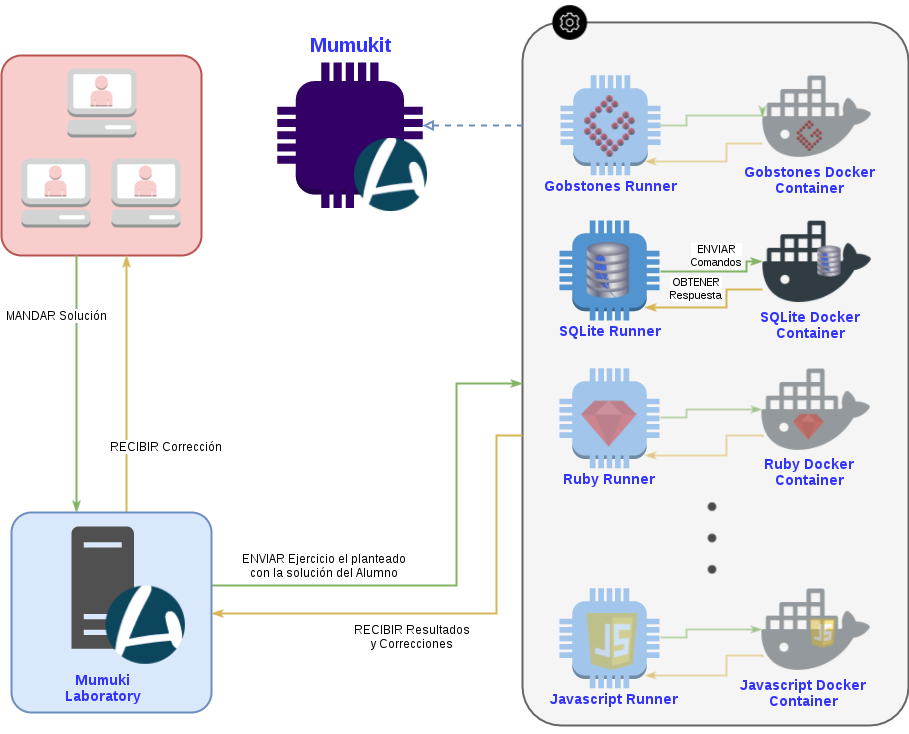
\includegraphics[width=\textwidth]{img/MQL-Arquitectura}
  \caption{Arquitectura MQL}
  \label{fig:arquitectura}
\end{figure}

En la figura~\ref{fig:arquitectura} se muestra el flujo de interacción
desde que el alumno envía la solución de un problema hasta que obtiene
la corrección.

Cada \textit{Runner}, al usar Mumukit, provee una interfaz HTTP con 3 rutas posibles

\begin{itemize}
    \item \texttt{GET /info}: retorna metada del runner
    \item \texttt{POST /query}: ejecuta una sentencia en particular
    \item \texttt{POST /test}: ejecuta todo el ejercicio
\end{itemize}

Cuando el alumno envía la solución, se ejecuta una petición
\texttt{POST /test} con todo el ejercicio completo (la solución
del alumno y lo preestablecido por el docente). Mumukit
recibe la petición y ejecuta al \textit{Runner} correspondiente,
el cual debe cumplir con ciertos métodos. El \textit{Runner}
adapta el ejercicio e interactúa con \textit{Docker} para
ejecutar el ejercicio y poder responder con la evaluación.


\subsection{Trabajo Realizado y Stack Tecnológico}

La elección del stack estuvo mayormente definida por las necesidades
de Mumukit. El \textit{Runner} debe está escrito en \textit{ruby}
y se creó un \textit{container Docker} con un motor SQL instalado.
Se optó por utilizar \textit{SQLite} como motor SQL
por ser mucho más veloz que los motores utilizados en
la industria. Se optó por una herramienta versatil
que permita rápidamente concentrarse en los conceptos.

\paragraph{Docker} funciona creando y destruyendo
máquinas virtuales de forma muy rápida y económica.
Este aspecto es muy útil ya que permite garantizar
que cada solución enviada por cada alumno a un
mismo \textit{Runner} sea ejecutada de forma aislada
y en un ambiente limpio.

Esta interfaz permite que el docente pueda
generar de manera \textit{ad-hoc} y personalizable
a cada ejercicio la configuración de base
para que un alumno pueda trabajar enfocándose
en el aprendizaje del concepto.

Las peticiones entre el \textit{Runner} y el \textit{worker}
se dan mediante datos con formato \textit{json}.
Mumukit permite configurar que la petición hacia el \textit{worker}
sea mediante un comando que recibe un archivo como parámetro.
El \textit{Runner SQLite} transforma el ejercicio en una estructura
del tipo:

\begin{listing}[ht]
    \begin{minted}[frame=lines,framesep=5mm,baselinestretch=1.2,
    bgcolor=light-gray,fontsize=\small]{json}

    {
        "init": "CREATE TABLE ...; CREATE ...;",
        "solution": "SELECT ... FROM ...;",
        "student": "SELECT * FROM table;",
        "datasets": ["INSERT INTO ....; INSERT INTO ...", "INSERT ....;"]
    }
    \end{minted}
    \caption{\textbf{JSON} enviado al \textit{worker}}
    \label{listing:yaml}
\end{listing}

El \textit{worker} utiliza un script en \textit{python}
para ejecutar el código del alumno y el del docente
en el DDL planteado para cada set de datos.
La respuesta esperada por \textit{Mumukit} es un \texttt{buffer}
de datos en el \texttt{stdout} junto al \texttt{exit code}.

Cuando la ejecución no contiene errores de sintaxis
y puede ser procesada por el motor, genera un \textit{dump} en formato \textit{json}
con las claves \texttt{solutions} y \texttt{results},
que contienen los \textit{rows} obtenidos como resultado de ejecutar
cada respectiva \textit{query} en cada set de datos provisto.
Esos resultados son procesados por el \textit{Runner} que evalúa
a posteriori la correctitud de la solución del alumno y
retorna un \textit{feedback} acorde.


\begin{figure}[h]
  \centering
  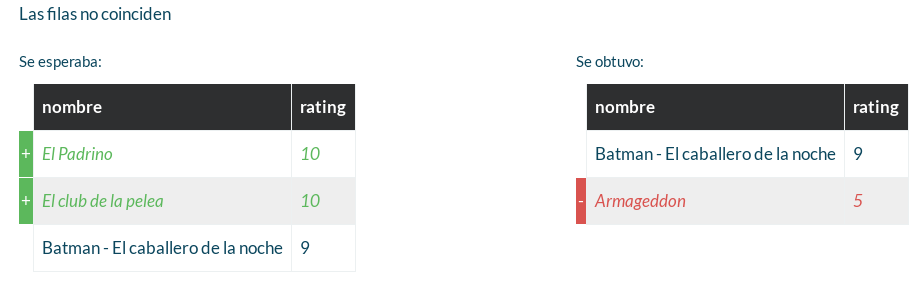
\includegraphics[width=\textwidth]{img/rows-error}
  \caption{Solución incorrecta}
  \label{fig:rows-error}
\end{figure}


\subsection{Retrospectiva}

Este trabajo se realizó mediante la modalidad
\textit{Taller de Trabajo de Inserción Profesional}.
Esta modalidad tiene un semestre de tiempo de vida
y es coordinada por un profesor de la carrera.
El siguiente es un detalle de las entregas acordadas
como plan de trabajo a lo largo de la cursada.

\subsubsection{Presentación del Proyecto}

Para la presentación del Proyecto MQL se generó cierto
trabajo de base que consistió en definir un backlog de tareas,
priorizarlas y estimarlas, generar el repositorio con
el stack tecnológico funcionando y hacer la presentación.

\subsubsection{Prueba de concepto}

\begin{itemize}
    \item Investigación sobre Docker y armado inicial del \textit{worker}
    \item Integración con Travis CI
    \item Integración con CodeClimate
    \item Primer borrador de este documento
    \item Ejercicio base con sintaxis inválida, detectando el fallo
          y mostrando la respuesta correcta.
    \item Ejercicio base correcto, verificando que los
          resultados retornados sean los deseados
\end{itemize}

\subsubsection{Entrega 1}

\begin{itemize}
    \item Modificación del script del \textit{worker} agregando soporte
    para ambas soluciones: la del alumno y la provista por el docente.
    \item Investigación sobre el funcionanmiento de los \textit{Hooks} de Mumukit.
    \item Modificación de ejercicios: se establece que el código inicial
    sea el obtenido de la variable asociada al campo \texttt{extra\_code}
    utilizado por el docente para la configuración inicial.
\end{itemize}

\subsubsection{Entrega 2}

\begin{itemize}
    \item Refactorización de \textit{worker} y \textit{Runner}.
    Se mejora la comunicación y se establecen mejores condiciones para el
    postprocesamiento de la solución.
    \item Se generan fixtures para tests de verificación correcta.
    \item Se generan fixtures para tests de casos de error.
    \item Generación de Test de Integración con la plataforma.
    \item Instalación de Mumuki Laboratory en forma local.
    \item Generación de un Capítulo SQL con ejercicios en Mumuki Laboratory local
\end{itemize}

\subsubsection{Entrega 3}

\begin{itemize}
    \item Refactorización del \textit{worker}.
    Se cambia la estructura de datos por formato \textit{json} en ambos sentidos
    de las peticiones.
    Se establecen mejoras en el procesamiento de datos.
    \item Refactorización del \textit{Runner} para que utilice el \textit{Checker}
    de \textit{Mumukit}. Esto permite desacoplar y delegar el análisis
    y la correción a otro componente que cumple esa única tarea.
    \item Refactorización completa de la comparación de los resultados del \textit{worker}.
    \item Codificación del \textit{Render HTML} para un \textit{feedback} adecuado.
    \item Definición de un ejercicio con mayor complejidad y múltiples datasets.
\end{itemize}

\subsubsection{Entrega 4}

\begin{itemize}
    \item Coloreo de sintaxis.
    \item Pull Request y correcta integración con Proyecto Mumuki en producción.
    \item Corrección de error que no permitía el encoding correcto.
    \item Corrección de error que no permitía que un resultado sea vacío.
    \item Refactorización de la estructura utilizada por docente al cargar un ejercicio.
    Se establece formato YAML para brindar mayor flexibilidad en el ejercicio.
    \item Se agrega al formato YAML la posibilidad de establecer el dataset
    esperado en lugar de la query dada como solución.
    \item Se agrega parseo mediante \texttt{diff}.
    \item Refactorización \textit{Render HTML} para colorear el \texttt{diff}.
    \item Versión final de este documento.
    \item Armado de presentación y demo.
\end{itemize}
